\documentclass[10pt, a4paper]{article}
\usepackage[utf8]{inputenc}
\usepackage[czech]{babel}
\usepackage[left=1.5cm,text={18cm, 25cm},top=2cm]{geometry}
\usepackage{graphicx}
\usepackage{titlesec}
\usepackage{multicol}
\usepackage{dirtree}
\setlength{\parskip}{0pt}

\title{Programování zařízení Apple\\ {\large 2.\,projekt -- Aplikace na zkoušení slovíček} }
\author{Petr Freyburg (xfreyb00)}
\date{}

\begin{document}

\maketitle

\section{Motivace}

Aplikace na zkoušení slovíček \textbf{IZAwords} slouží na přezkušování slovíček při učení se cizího jazyka. Typickým uživatelem je žák/student nějaké formy vzdělávání v~cizím jazyce, který se například potřebuje připravit na test. Aplikace mu má umožnit definovat si lekce slovíček a~z~těchto slovíček být přezkušován, například při cestě do školy vozidlem městské hromadné dopravy.

Hlavní cílem uživatele této aplikace je procvičit se, repspektive zdokonalit se, v~cizím jazyce.

\section{Používání aplikace}

Po otevření aplikace se uživateli zobrazí seznam lekcí, zde si může buď přidat novou lekci nebo si vybrat některou ze stávajících.

Při výběru stávájící lekce se uživateli zobrazí detaily dané lekce. Uživatel může změnit název lekce, otevřít seznam slovíček nebo se pustit do zkoušení, zkoušení se ovšem spustí pouze v~případě, že jsou již v~lekci uloženy nějaká slovíčka. Seznam lekcí a~detail lekce jsou na obrázku \ref{lekce}.

Při otevření seznamu slovíček, uživatel může přidávat a~odebírat, ale také editovat stávající. Když uživatel přidává nové slovíčko nebo edituje stávající, v~detailu slovíček určí český a~anglický překlad slovíčka.

Při zkoušení se zamíchaný seznam slovíček zobrazí horizontálně, mezi slovíčky se lze přesouvat zleva doprava a~naopak, lze se libovolně vracet. Ke každému slovíčku je přiřazen jeden textový vstup.

Při klepnutí na tlačítko \uv{Vyhodnotit} se zobrazí vyhodnocení daného testu. Zobrazí se počet špatně zodpovězených slovíček a~kolik z~nich nebylo vyplněno vůbec. Je možné si vyhodnocovat test průběžně po každém vyplněném slovíčku, cílem není uživateli zabránit vyplňovat test po stisknutí daného tlačítka, ale umožnit mu způsob učení, který vyhovuje jemu samému. Zkoušení a~vyhodnocení jsou na obrázku \ref{zkouseni_vyhodnoceni}.

\section{Data}

Data aplikace jsou uloženy v~\verb|CoreData|. Jednotlivá uživatelská data a~vazby mezi nimi jsou znázorněny na obrázku \ref{data}.

\begin{figure}[h]
\centering

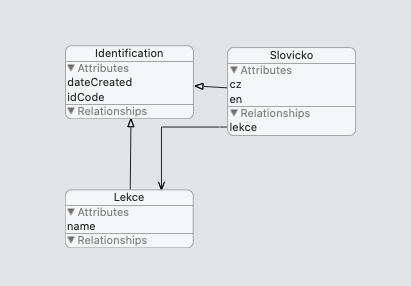
\includegraphics[width=0.4\textwidth]{img/data.png} 
\caption{Data aplikace.}\label{data}
\end{figure}

\section{Implementační detaily}

Aplikace je postavená na demostrační knihovně \verb|MHCoreData|, použita byla i~demonstrační aplikace. Bylo použito \verb|SwiftUI|.

Seznamy lekcí a~slovíček vycházejí z~demonstrační aplikace. Při spuštění zkoušení z~detailu lekce se nejdříve připraví všechna slovíčka dané lekce, podle zvoleného typu zkoušení (z~češtiny do angličtiny nebo z~angličtiny do češtiny) se předá pole textových řetězců s~textem slovíček ve vybraném jazyce pro zobrazení. Dále se předává pole všech slovíček (s~oběma překlady) a~název lekce pro zobrazení.

Po klepnutí na vyhodnocení testu se do třídy \verb|VyhodnoceniVC| předává slovník odpovědí ve tvaru \verb|dotaz| $\rightarrow$ \verb|odpoved|, pole všech slovíček a~typ zkoušení. Samotné vyhodnocení probíhá v~metodě \verb|provest|. Nejdříve je vytvořen čítač špatných odpovědí a~čítač nezodpovězených. Oba jsou nastaveny na počet slovíček. Podle typu zkoušení se cyklí všechna slovíčka v~příslušném jazyce dané lekce a~pokud se vyskytují ve slovníku odpovědí, je snížen čítač nezodpovězených, pak se porovnává zda odpověď souhlasí s~uloženým překladem. Když souhlasí je snížen i~čítač špatných odpovědí.

Tato metoda vrací strukturu \verb|Vyhodnoceni|, do které jsou vloženy ony dva čítače a~pole struktur \verb|zodpovezene_slovicko|, které obsahuje otázku, uživatelovu odpověď a~spravnou odpověď. V~tomto poli jsou pouze informace o~špatně zodpovězených slovíčkách. Struktura s~informace o~vyhodnocení je poté předána k~zobrazení ve vyhodnocení.

\subsection{Soubory aplikace}

\begin{figure}

\dirtree{%
	.1 System files/.
	.1 Tabulky, pohledy, UI/.
	.2 MainVC.swift .
	.2 Lekce-VC.swift .
	.2 Vyhodnoceni-VC.swift .
	.2 Slovicko-VC.swift .
	.2 Zkouseni.swift .
	.2 About.swift .
	.2 Vyhodnoceni.swift .
	.1 Model-CD-classes/ .
}

\caption{Soubory aplikace.}\label{files}


\end{figure}

Na obrázku \ref{files} jsou znázorněny soubory aplikace. Soubory končící \verb|-VC.swift| jsou \emph{View Controllery}. \verb|Zkouseni.swift|, \verb|Vyhodnoceni.swift| a~\verb|About.swift| obsahují SwiftUI struktury pro zobrazení.

\begin{figure*}
\begin{center}
\begin{multicols}{2}

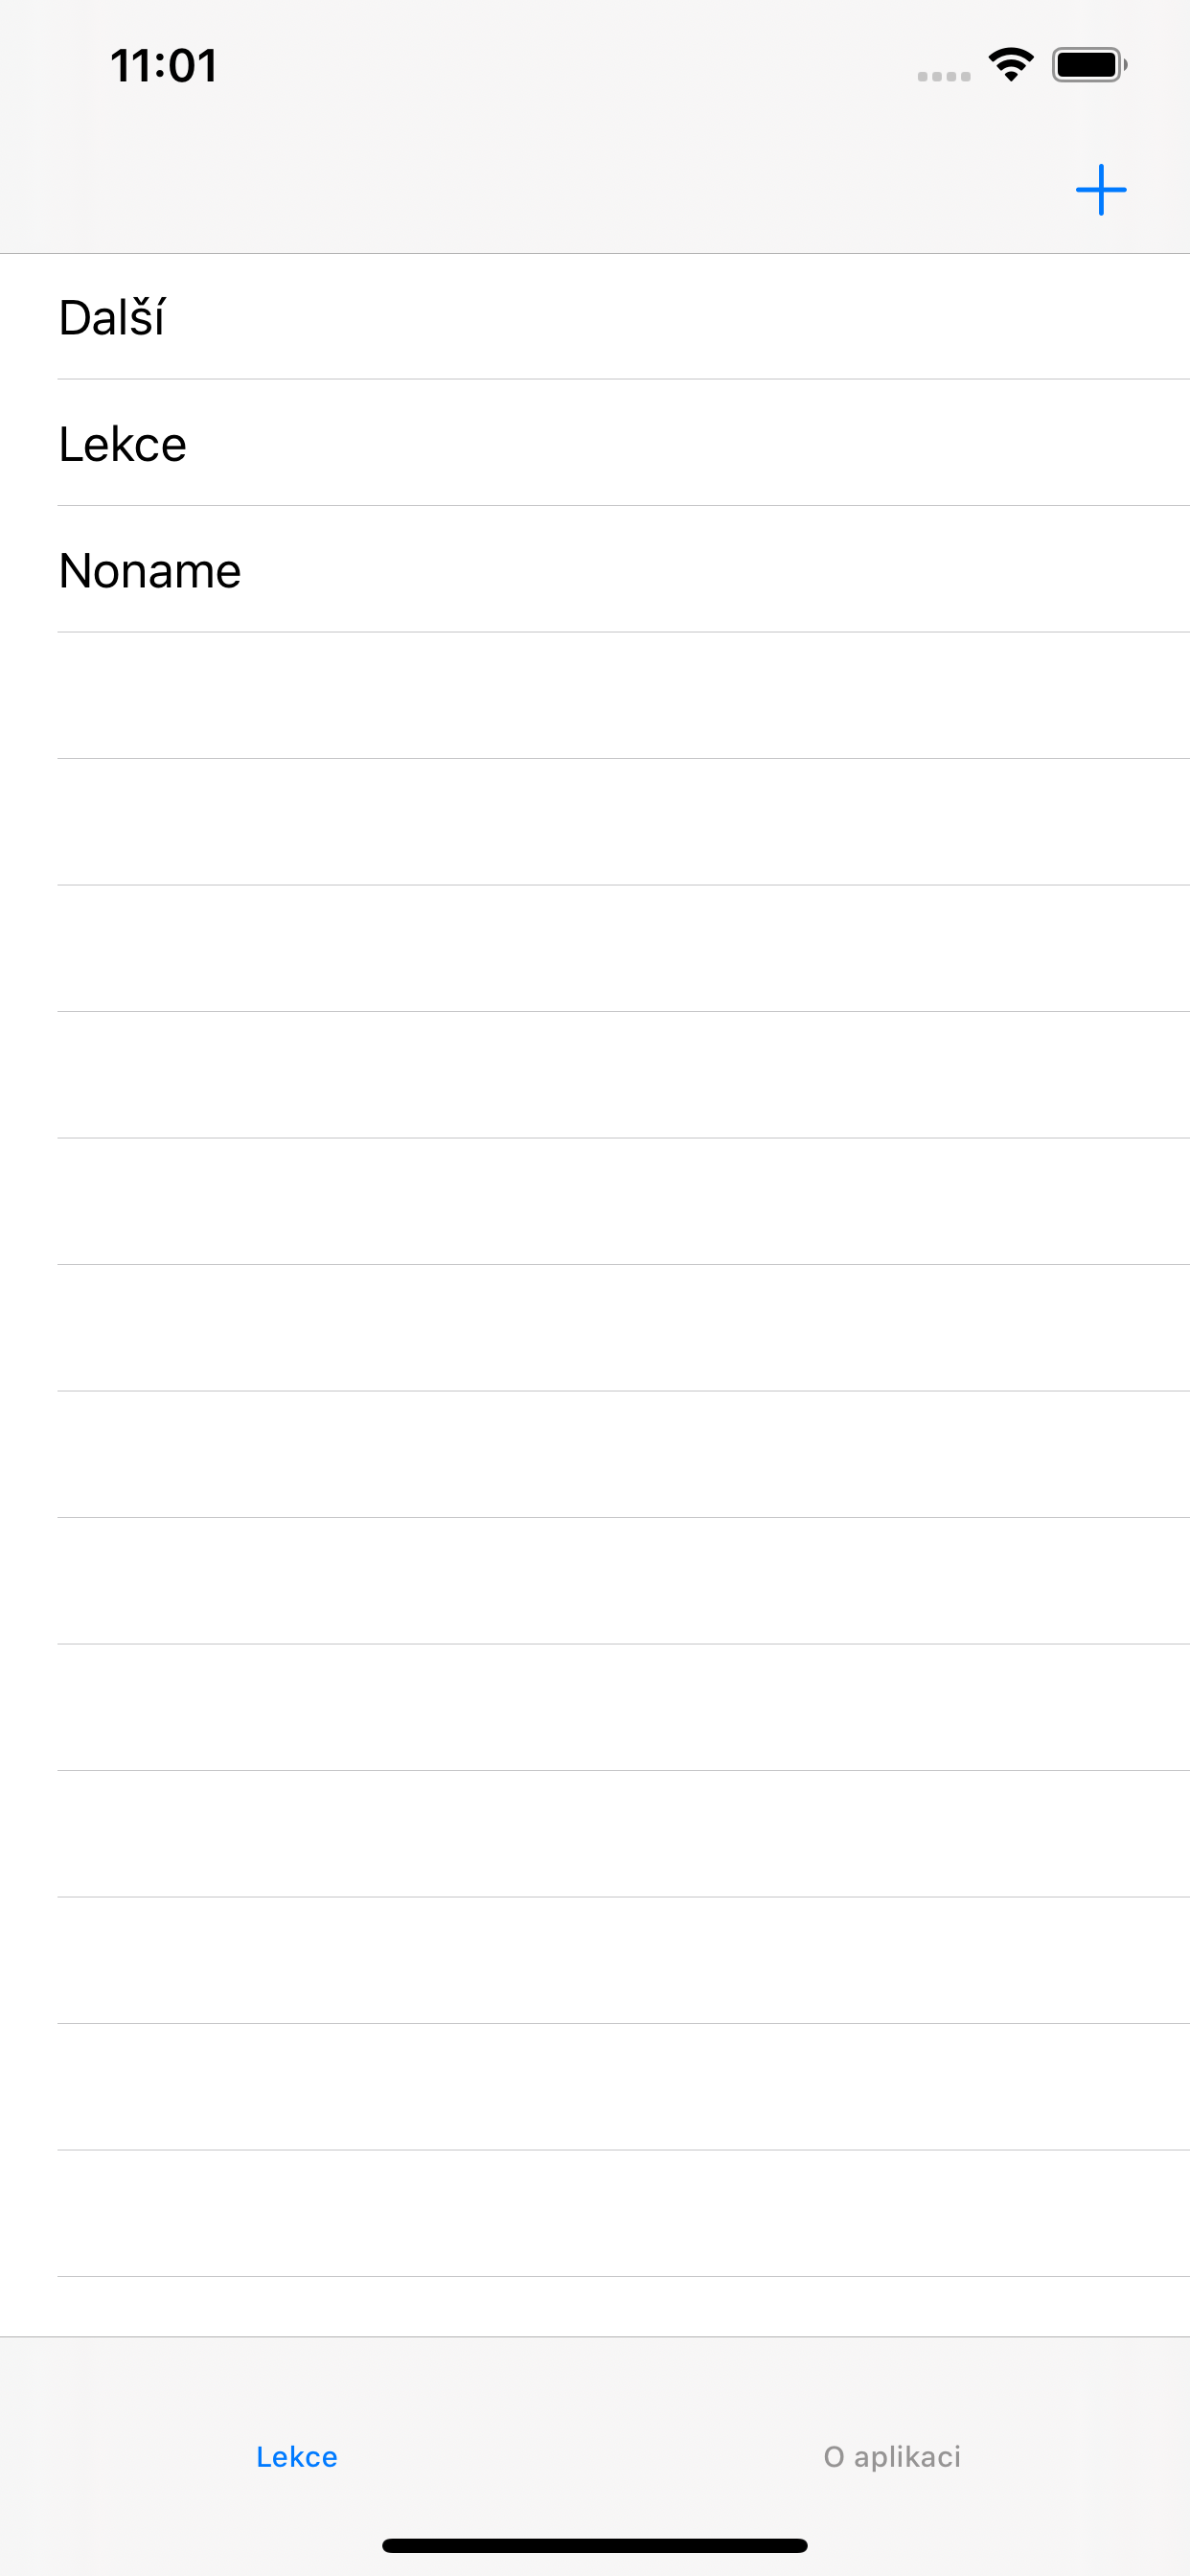
\includegraphics[width=0.25\textwidth]{img/lekce.png} \par
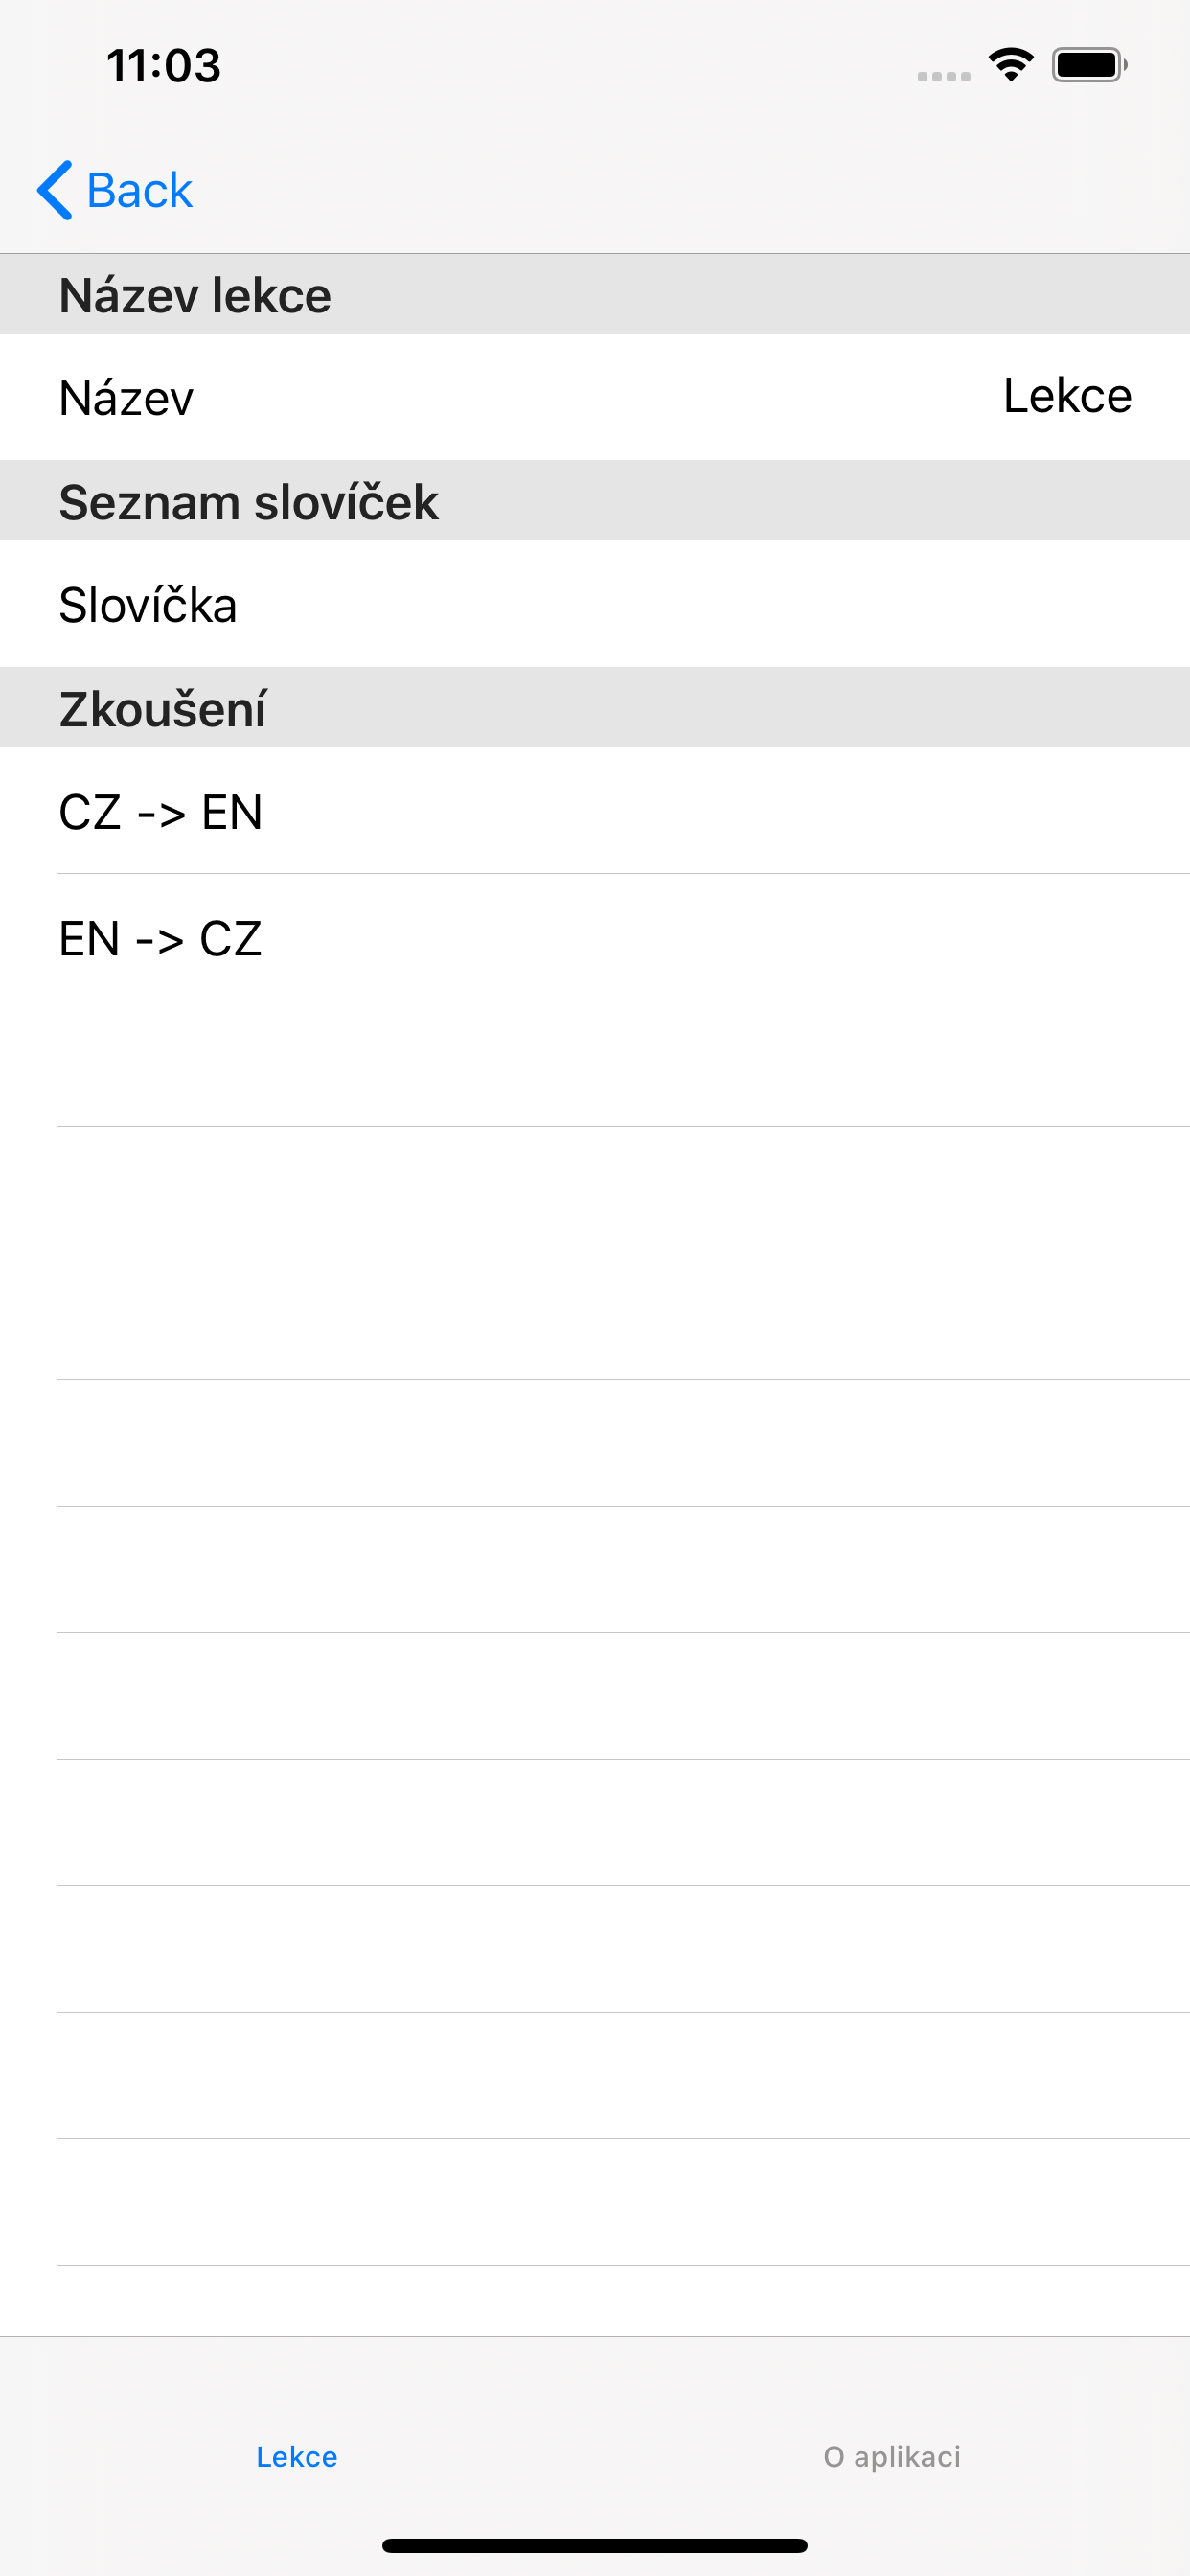
\includegraphics[width=0.25\textwidth]{img/lekce-detail.png} \par

\end{multicols}
\caption{Seznam lekcí a detail lekce} \label{lekce} 
\end{center}
\end{figure*}

\begin{figure*}
\begin{center}
\begin{multicols}{2}

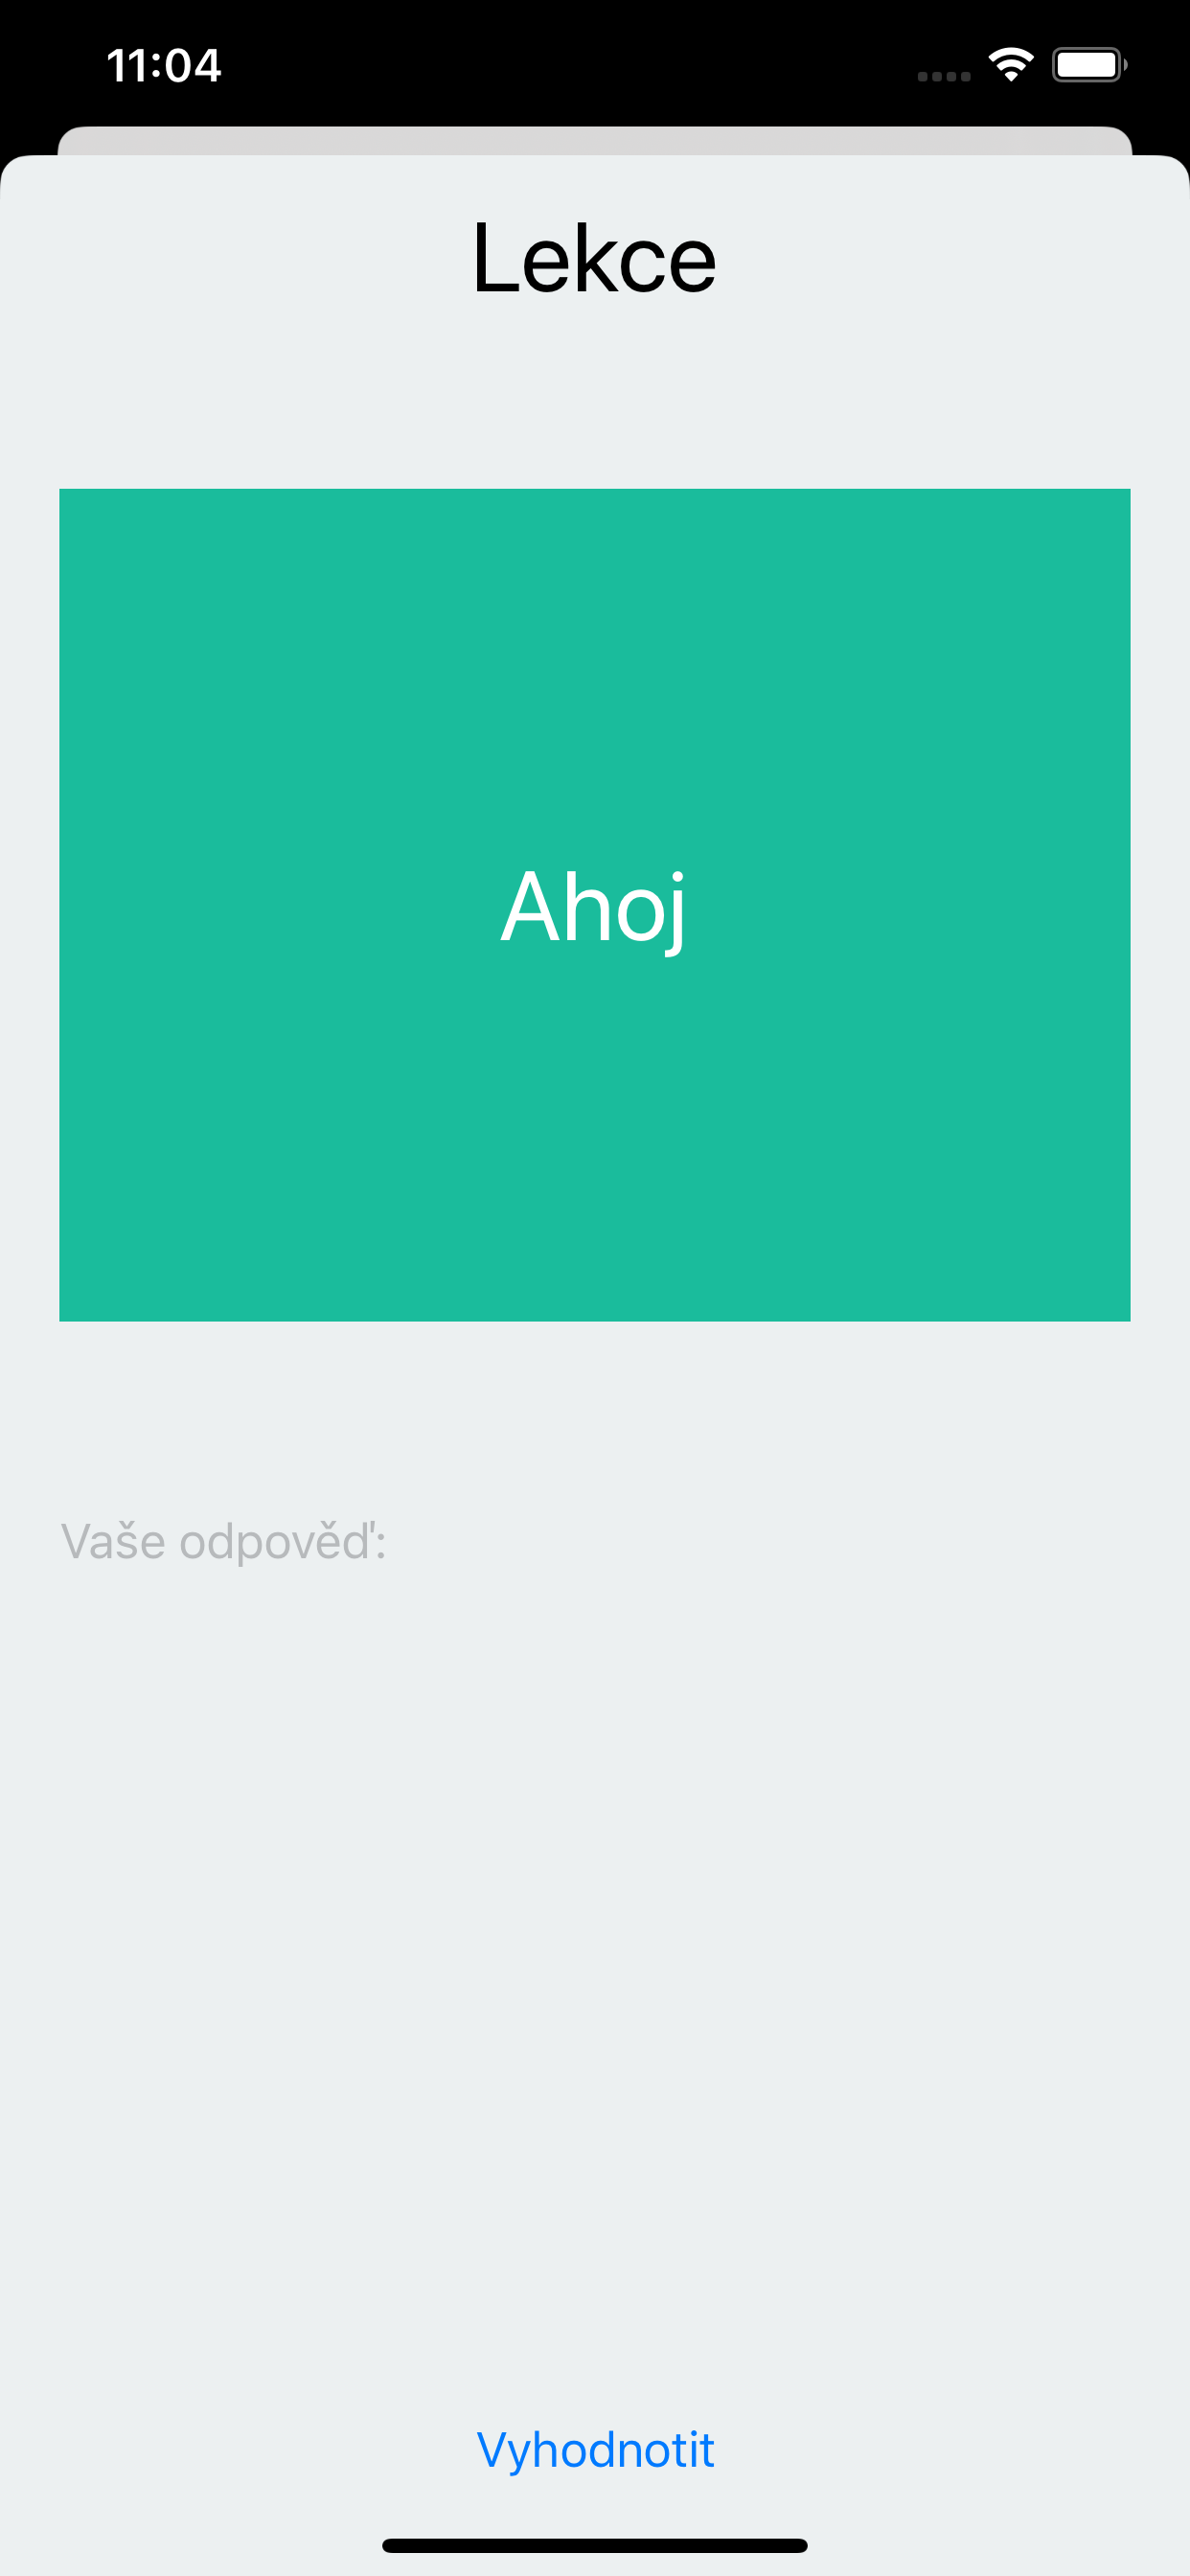
\includegraphics[width=0.25\textwidth]{img/zkouseni.png} \par
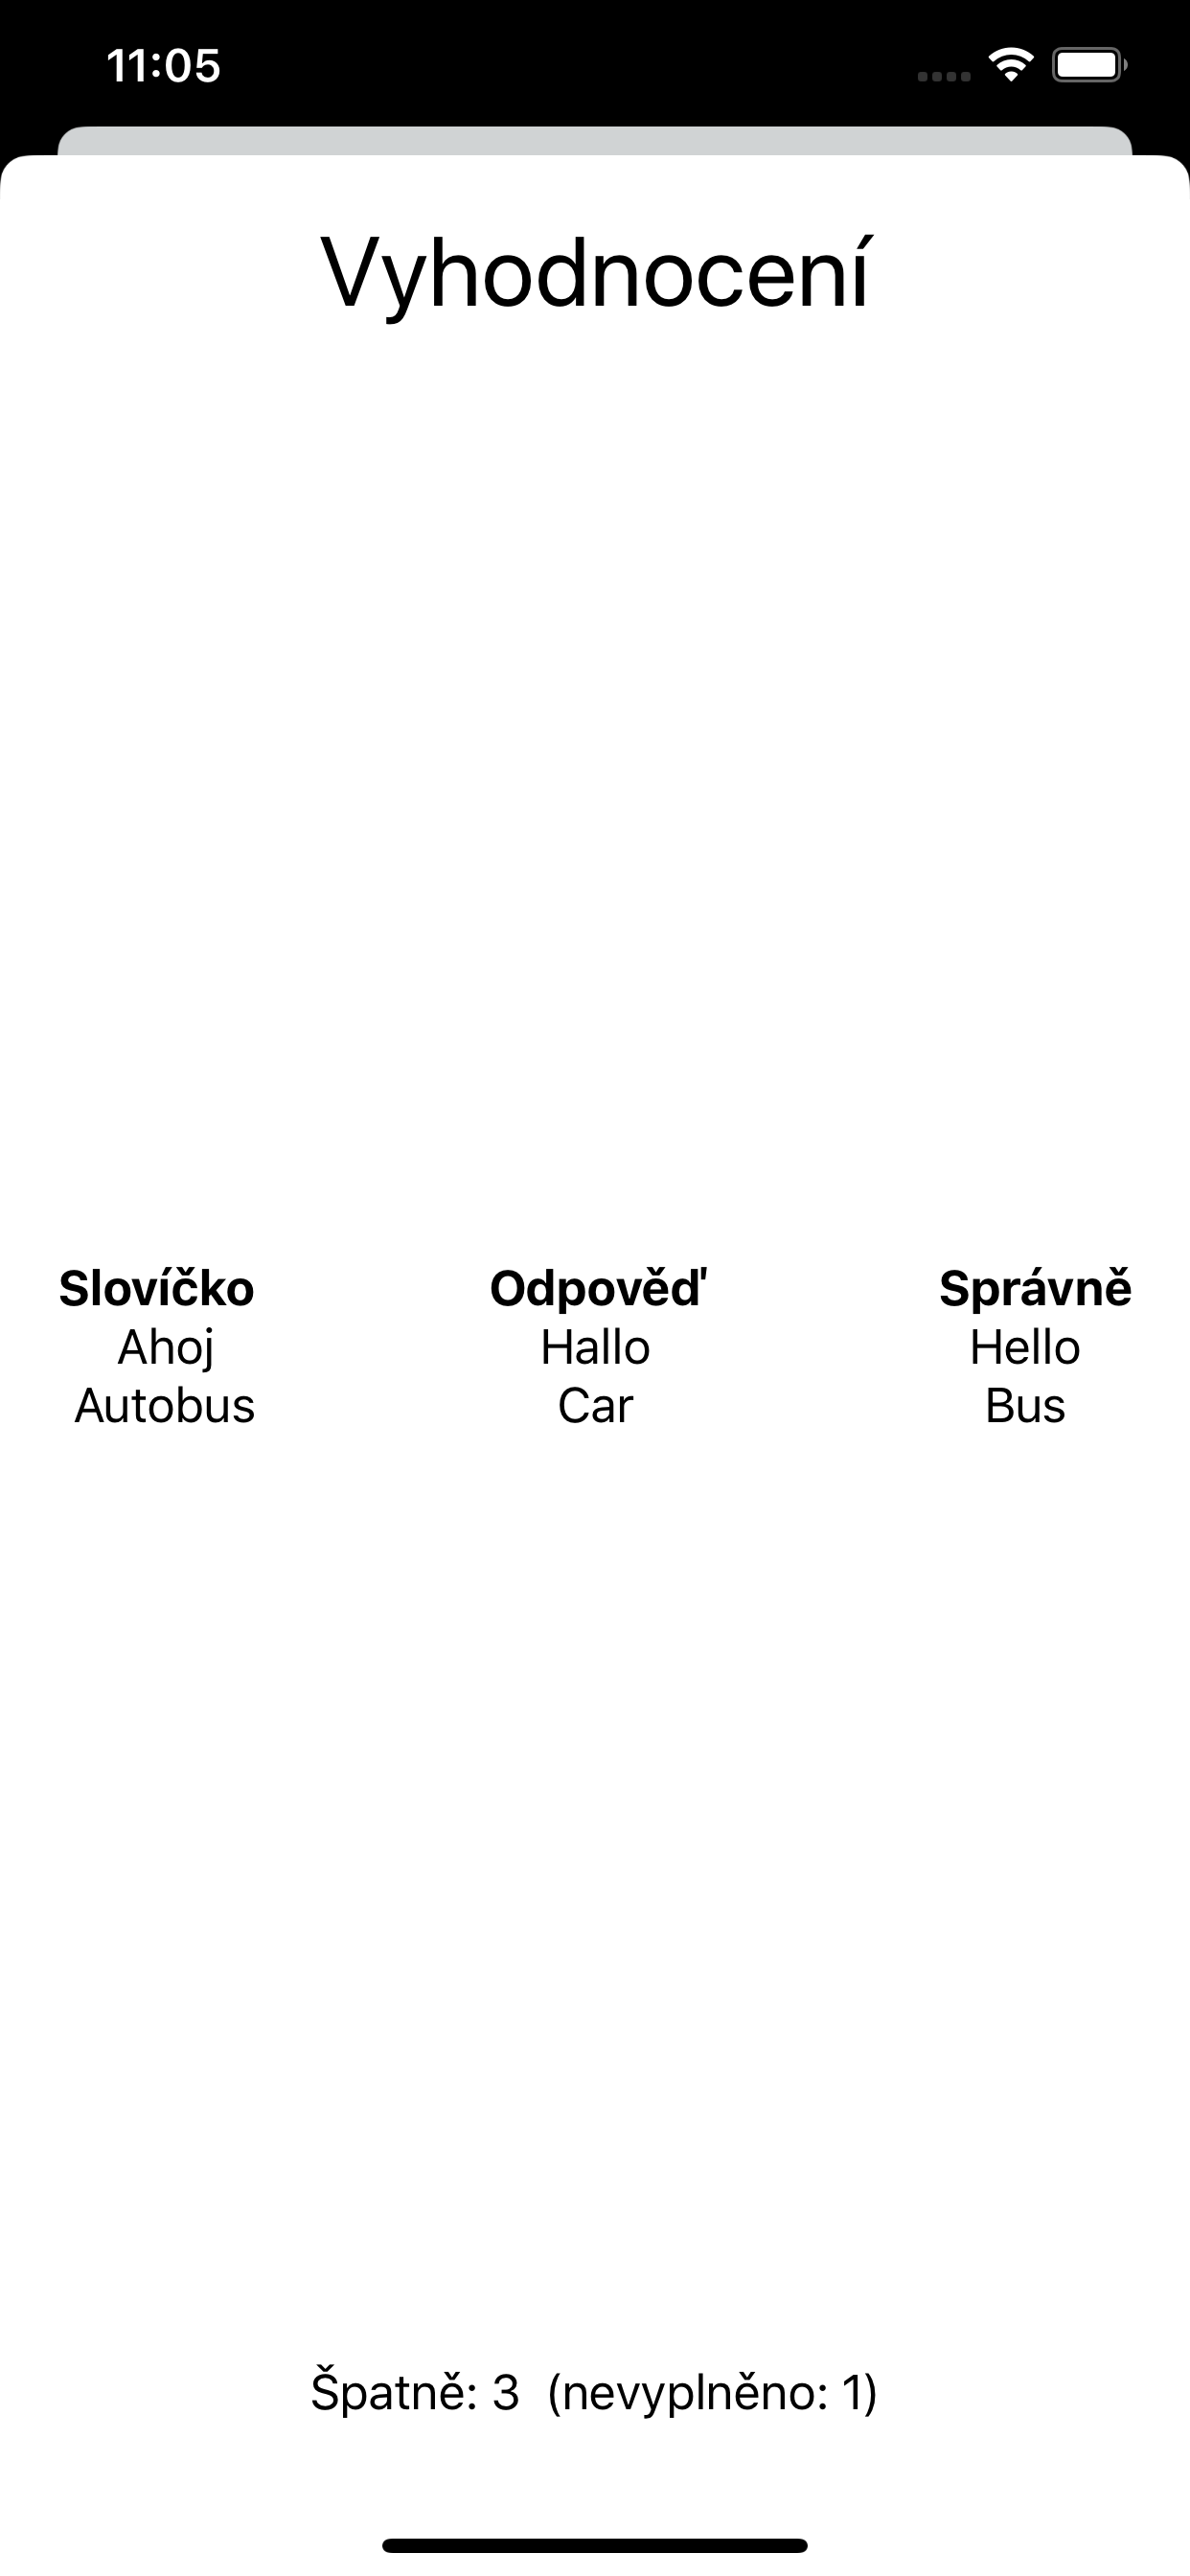
\includegraphics[width=0.25\textwidth]{img/vyhodnoceni.png} \par

\end{multicols}
\caption{Zkoušení a vyhodnocení zkoušení.} \label{zkouseni_vyhodnoceni} 
\end{center}
\end{figure*}

\end{document}
